\chapter{双拐点暴涨模型}

前面的章节中我们讨论了在超引力中构造拐点暴涨模型。接下来我们将简要介绍双拐点
暴涨模型以及在超引力框架内的实现,并针对该模型
计算了诱导引力波的能谱,发现该引力波信号有望在将来被空间引力波探测实验所发现。

% 双拐点暴涨模型
\section{双拐点暴胀模型}
拐点暴胀通常指这样的暴胀模型,存在场值$\phi=\phi_0$(拐点)使得势能在该处的二阶导数为零
\begin{equation}
    V^{\dprime}(\phi_0) = 0
\end{equation}

势能的一般形式为

\begin{equation}
    \label{eq:inf_potential}
    V (\phi)=V_0+a (\phi-\phi_0)+\frac{c}{6}{\left(\phi-\phi_0\right)}^3\\
\end{equation}
\begin{equation}
    V_0\equiv V (\phi_0),\ a\equiv V' (\phi_0),\ c\equiv V^{\tprime} (\phi_0) 
\end{equation}

高阶项 $(n \geq 4)$ 被截断。相应的慢滚参数为
\begin{equation}
    \label{eq:psrp}
    \epsilon = \frac{M_p}{2}\left(\frac{V'}{V}^2\right),\ \eta=M^2_p
    \left(\frac{V^{\dprime}}{V}\right),\ \xi^2=M^4_p\left(\frac{V'V^{\tprime}}{V^2}\right)
\end{equation}

接下来通过WMAP、Planck等实验观测到的标量扰动大小$\mathcal{P}_R$和标量谱指标$n_s$来确定系数a和c。
令暴胀结束时的场值为$\phi_e$,那时有$\epsilon\sim
1$。则对应$\phi\sim\phi_e$的e-folding数为
\begin{align}
    \label{eq:e-folding}
    \mathcal{N} &= \frac{V_0}{M^2_p}\sqrt{\frac{2}{ac}}\lbrack
    F_0(\phi_e)-F_0(\phi)\rbrack \\
    F_0(z) &= \cot^{-1}\left(\sqrt{\frac{c}{2a}}(z-\phi_0)\right)
\end{align}

如果将慢滚参数在极值处的平方根定义为 $X$, $\mathcal{N}$ 中涉及 $\phi$
的部分定义为 $Y$,那么可以将各慢滚参数及可观测量用统一用$X,Y$进行描述。

\begin{align}
    \epsilon &=
    \frac{2V_0^2}{c^2M_p^6\mathcal{N}^4} {\left(\frac{Y}{X} \right)}^4 \\
    \eta &=
    -\frac{2}{\mathcal{N}}\frac{Y}{S}\left(\sqrt{1-X}\cos Y-\sqrt{X}\sin
    Y\right)\\
    \xi^2 &= \frac{2}{\mathcal{N}^2}{\left(\frac{Y}{X}\right)}^2
\end{align}

在暴胀期间,$\epsilon \ll 1$,导致$X=S\sqrt{\epsilon}\leq\sqrt{\epsilon}\ll
1$,故而有$S\approx \sin Y$。相应的功率谱,标量谱指标及其跑动为
\begin{align}
    \mathcal{P}^{1/2}&\equiv\frac{1}{\sqrt{24\pi^2}}\frac{V_0^{1/2}}{\epsilon^{1/2}M_p^2}
    \approx\frac{V_0^{1/2}}{2\sqrt{6}\pi M_p^2 X}\sin^2Y\\
    n_s&\equiv1+2\eta-6\epsilon\approx1-\frac{4}{\mathcal{N}}Y\cot Y\\
\end{align}

% 双拐点暴涨模型在超引力中的实现
\section{在超引力中单场构造双拐点暴胀模型}
在第三章中曾提到在超引力中构造暴胀模型通常采用双场理论。通常我们期望暴胀过程中
演化方程只涉及暴胀场,因而要求其它的标量场稳定在使势能取极值处。
在某些模型中,需要特别注意辅助场$S$在$s=0$处的稳定性。
有两种方法可以做到,一是在K\"ahler势中添加项$S\bar{S}$,二是选择不含标量自由度
的手征场$S$作为辅助场。后一种方法中涉及描述宇宙演化的只有一个无约束的手征超场$\Phi$场。
基于此,产生了一类无需引入额外非约束手征超场就能描述当前宇宙演化的暴胀模型
\citep{kallosh2015inflation,dall2014sgoldstino,linde2015does} 。


后来,Ketov和Terada提出了一类基于单手征超场$\Phi$的新暴胀理论
\citep{ketov2014generic,ketov2014inflation}。在 \citep{ketov2014generic}
中,提出了一种新的对数形式的K\"ahler势
\begin{equation}
  \label{eq:logarithmic-kahler-potential}
  K =
-3\ln \left[1+\frac{\Phi+\bar{\Phi}+\zeta{\left(\Phi+\bar{\Phi}\right)}^{4}}{\sqrt{3}}\right].
\end{equation}
$\zeta$是常系数。其中超场$\Phi$通常被分解为实部$\phi$和虚部$\chi$
\begin{equation}
  \Phi = \frac{1}{\sqrt{2}}(\phi+i\chi). 
\end{equation}
由于该K\"ahler势在shift变换$\Phi\rightarrow
\Phi+iC$下是不变的,超场$\Phi$的虚部$\chi$不会出现在K\"ahler势中,因此可以作为
暴胀场的候选者。在这个K\"ahler势中,四次方项的作用是在暴胀过程中将场$\phi$
稳定在零附近。并且K\"ahler势中并没有加入平方项和三次方项,尽管这些项不破坏对称
性,但是相应的系数可以通过调节超场$\Phi$和其它超场之间的耦合而压低。

不论超势取何种形式,当K\"ahler势取$(\ref{eq:logarithmic-kahler-potential})$式时,场$\Phi$的动能项系数为
\begin{equation}
  \label{eq:kinetic-coefficient-of-Phi}
  G(\phi,\chi) =
  \frac{3(1+32\zeta^2\phi^{6}-8\zeta\phi^2(3\sqrt{3}+\sqrt{2}\phi))}{{\left(\sqrt{3}+\sqrt{2}\phi+4\zeta\phi^{4}\right)}^2}.
\end{equation}

\begin{figure}[!http]
  \centering
  \includegraphics[width=5in]{Img/kinetic_coefficient_for_Phi.png}
  \caption{$\zeta=1$时,手征场$\Phi$的动能项系数与$\phi$的函数关系}\label{fig:kinetic-coefficient_for_Phi}
\end{figure}

从图$(\ref{fig:kinetic-coefficient_for_Phi})$可知,为了使$G>0$,$\phi$被限制在一
个有限的区间内。$\zeta$越大,$\phi$的取值区间越窄。因而在暴胀期间,标量场$\phi$的影响可以忽略,势能近似为暴胀场$\chi$的函数,K\"ahler势中四次方项的调节作用
在这里清晰地体现出来了。当超势为
\begin{equation}
  W = \frac{1}{\sqrt{2}} f(-\sqrt{2}i\Phi),
\end{equation}
时,其中$f$为实函数,沿暴胀场方向的势能为
\begin{equation}
  V\simeq {\left[f^\prime(\chi)\right]}^2.
\end{equation}
暴胀结束后,场朝着全局最小值滚去,最终得到一个超对称闵可夫斯基真空。这种情况对一
大类的超势都成立,同时也期望能在此基础上通过对K\"ahler势作一个微小的修正,能够抬升真空能得到dS真空。然而no-go定理\citep{kallosh2014analytic}告诉我们对K\"ahler势和超势作一个无穷小修改,无法将具有超对称的闵可夫斯基真空连续地变化到dS真空。举一个例子,当超势取如下形式时
\begin{equation}
  W=m(c\Phi+1),  
\end{equation}
$c$和$d$为实参数,在$\phi=0$方向上势能为
\begin{equation}
  V(\phi=0,\ \chi)=m^2c(c-2\sqrt{3}) 
\end{equation}
\begin{figure}
  \centering
  \includegraphics[width=5in]{Img/potential-for-linear-superpotential.png}
  \caption{蓝实线为数值计算得到的暴胀场的演化过程,红虚线为有效势能的绝热近似。黑实线为势能$V(\phi(\chi),
  \chi)$的对数等高线。当暴胀场靠近吸引子解前以及暴胀结束后都有一个震荡阶段。}\label{fig:potential-for-linear-superpotential}
\end{figure}
显然参数$c$的大小将决定势能大于零还是小于零。更具体的分析会发现,暴胀发生的过程并不完全在$\phi=0$方向。从图$(\ref{fig:potential-for-linear-superpotential})$中可以
看到,暴胀结束后得到的是一个超对称破缺的闵可夫斯基真空。通过对参数$c$进行微小的调节就能得到预期的德$\cdot$西特宇宙,$V_0\sim
10^{-120}$。但是代价为引起了强超对称破缺,得到的引力微子质量$m_{3/2}$比通常理论预期的TeV量级高出多个量级。当考虑到粒子物理标准模型的时候,暴胀结束后是否恢复超对称性是一件很重要的事情。例如\citep{endo2006moduli,nakamura2006gravitino,kawasaki2006gravitino,kawasaki2006gravitino-overproduction,asaka2006gravitinos}指出当真空超对称破缺时,早期宇宙中从暴胀场衰变得到的引力微子数目会增多,而这将引起灾难。另外\citep{degrassi2012higgs}中指出如果超对称破缺的能标过高,电弱真空会遇到稳定性问题。

为了规避上述困难,同时不破坏no-go定理的前提下,有两种方法既能抬升真空势能得到德$\cdot$西特真空又能避免大的超对称破缺。一是引入额外的手征多态(Polonyi场),并且对其施加强约束尽可能降低其对宇宙演化的影响\citep{dudas2013strong}。另一个方法是引入零幂手征超场\citep{ferrara2014cosmology,kallosh2015inflation,dall2014sgoldstino,kallosh2015inflation-de-sitter,linde2015does},并且能从弦论中找到理论解释\citep{kallosh2014emergence}。

沿着这个思路,\citep{ketov2016susy}讨论了暴胀结束后恢复超对称性的条件,以及通过添加一个满足零幂条件$S^2=0$的Polonyi超场作为超对称破缺场$S$来控制超对称破缺的能标。


仍然考虑带有平移对称性的K\"ahler势\citep{ketov2016susy}
\begin{align}
    K=ic(\Phi-\bar\Phi)-\frac{1}{2}{(\Phi-\bar\Phi)}^2-\frac{\zeta}{4}{(\Phi-\bar\Phi)}^4,
\end{align}
其中$c$和$\zeta$为实参数。暴胀场取为手征超场$\Phi=(\phi+i\chi)/\sqrt{2}$的实部分量$\phi$。只要四次方项$\frac{\zeta}{4}{(\Phi-\bar\Phi)}^4$中的$\zeta$取得足够大,则暴胀场$\phi$在暴胀期间,场$\chi$的期望为$\langle\chi\rangle\approx0$。

参考了racetrack模型\citep{krasnikov1987supersymmetry,escoda2003saltatory,blanco2005racetrack}和其他模型\citep{ketov2016susy},我们选取如下形式的超势
\begin{align}
    W=a_0(1+a_1e^{-b_1\Phi}+a_2e^{-b_2\Phi}+a_3e^{-b_3\Phi}).
\end{align}

如果我们在宇宙学常数为零的真空中恢复来真空的超对称性(关于真空中的超对称破缺问题的讨论请参考文献\citep{gao2015inflection}),则F-term和势能V在$\Phi=0$处应当都为零,即$D_{\Phi}W=0$,$V=0$,这要求超势W满足约束条件
\begin{align}\label{eq:sp_constrain}
    W=\partial_{\Phi}W=0.
\end{align}
求解约束条件 (\ref{eq:sp_constrain}) 可以消去参数$a_1$和$a_2$
\begin{align}
    a_1\rightarrow \frac{b_2+a_3b_2-a_3b_3}{b_1-b_2},\qquad 
    a_2\rightarrow \frac{-b_1-a_3b_1+a_3b_3}{b_1-b_2}.
\end{align}
将K\"ahler势和超势代入到公式
\begin{align}
    V=e^{K/M^2_P}\lbrack
    D_{\Phi_i}W{(K^{-1})}^{ij^{*}}D_{\Phi^{*}_j}W^{*}-3M^{-2}_P|W|^2\rbrack,
\end{align}
中,可以得到标量势能$V(\phi)$。其中,
\begin{align}
    D_{\Phi}W=\partial_{\Phi}W+M^{-2}_P{(\partial_{\Phi}K)}W,
\end{align}
上两式中,$M_{P}^{2}=1 /8\pi G$。
以及K\"ahler度规的逆,
\begin{align}
    K^{ij*} = \frac{\partial^2K}{\partial\Phi_i\partial\Phi^{*}_j}.
\end{align}

当在参数空间中选取某组参数如
\begin{align}\label{eq:parameters}
    a_0 = 4.35\times 10^{-6},
    a_3 = 7\times 10^{-8},
    b_1 = 3.05,
    b_2 = 6.3868164,
    b_3 = -4.4,
    c = 2.8.
\end{align}
时,标量势能$V(\phi)$有两个近反射点,如图\ref{fig:potential}中所示。场取较大值处的拐点给出与当前CMB数据相一致的标量谱指标和张标比,较小值处的拐点可以使标量扰动的功率谱产生一个尖峰从而生成原初黑洞。
\begin{figure}[!htbp]
    \centering
    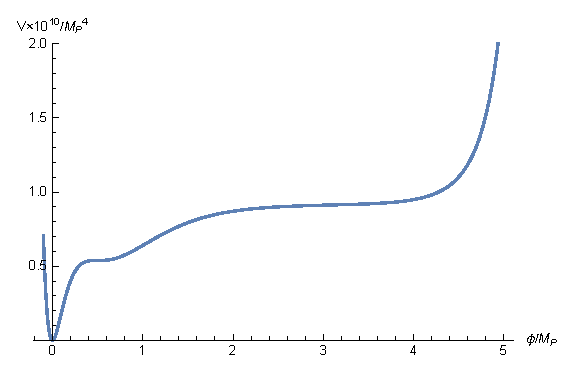
\includegraphics[width=5in]{Img/potential.eps}
    \caption{双拐点标量势能$V(\phi)$}\label{fig:potential}
\end{figure}

在FRW背景以及单场慢滚框架下,基于势能的慢滚参数$\epsilon_V$和$\eta_V$为
\begin{align}
    \epsilon_V &= \frac{1}{16\pi G}{\left(\frac{V^\prime}{V}\right)}^2, \\
    \eta_V &= \frac{1}{8\pi G} {\left(\frac{V^{\prime\prime}}{V}\right)}.
\end{align}

由于在拐点附近势能变得极端平坦,因此慢滚近似不再适用\citep{dimopoulos2017ultra,germani2017primordial},代之以极端慢滚暴胀。此时为了更精确地求解暴胀过程,势能慢滚参数需要替换为哈勃慢滚参数\citep{schwarz2001higher,leach2002cosmological,schwarz2004primordial},
\begin{align}
    \epsilon_H &= -\frac{\dot{H}}{H^2}, \\
    \eta_H &= -\frac{\ddot{H}}{2H\dot{H}}=\epsilon_H-\frac{1}{2}\frac{d \ln\epsilon_H}{dN_e}, \\
    \xi_H &=
    \frac{\dddot{H}}{2H^2\dot{H}}-2\eta^2_H=\epsilon_H\eta_H-\frac{d\eta_H}{dN_e},
\end{align}

其中,$N_e(t)$表示从视界穿过$k_{*}$到暴胀结束期间的e-folding数,通常在取值在范围$50\sim60$之间。

标量谱指标及其跑动和张标比的领头阶可以用$\epsilon_H,\eta_H,\xi_H$来表示
\begin{align}
    n_s &= 1- 4\epsilon_H+2\eta_H, \\
    \alpha &= \frac{dn_s}{d\ln k}=10\epsilon_H\eta_H-8\epsilon_H^2-2\xi_H, \\
    r &= 16\epsilon_H.
\end{align}

在参数集 (\ref{eq:parameters}),相应的数值结果为
\begin{align}
  n_s &= 0.9635,\\
  \alpha&=-0.00369,\\
  r&=0.00276,
\end{align}

当$k_{\star}=0.05Mpc^{-1}$时,在$68\%$的置信水平上与Planck
2018给出的对CMB的限制结果相一致\citep{akrami2018planck}
\begin{align}
  n_s &= 0.9640\pm 0.0043,\\
  \alpha &= -0.0071\pm 0.0068,\\
  r &< 0.079.
\end{align}

标量扰动的功率谱在慢滚暴胀模型通常用近似公式
\begin{equation}
  \label{eq:scalar-perturbation-power-spectrum}
  \mathcal{P}_{\mathcal{R}} = \frac{V}{24\pi^2M^2_P\epsilon_V}.
\end{equation}
计算得到。由于在拐点处,势能导数为零,因此使用势能慢滚参数的功率谱近似公式在
拐点处产生无穷大,导致公式失效。因而
\citep{germani2017primordial,motohashi2017primordial}中采用了不同的近似公式,
由于哈勃慢滚参数在整个暴胀期间始终大于零,因此基于哈勃慢滚参数的近似功率谱公式
\begin{equation}
  \label{eq:scalar-perturbation-power-spectrum-hubble}
  \mathcal{P}_{\mathcal{R}} \simeq
  \frac{1}{8\pi^2M^2_P}\frac{H^2}{\epsilon_H}.
\end{equation}
将会给出更准确的结果。不过仍然指出这种近似可能会导致对PBH的质量函数产生错误的
估计,因而 \citep{ballesteros2018primordial}中根据Mukhanov-Sasaki (MS)公式
\citep{sasaki1986large,mukhanov1988quantum}数值求解精确的功率谱。 
Mukhanov-Sasaki (MS)方程为
\begin{align}\label{eq:ms}
    \frac{d^2u_k}{d\eta^2}+\left(k^2-\frac{1}{z}\frac{d^2z}{d\eta^2}\right)u_k=0,
\end{align}
其中$\eta$为共形时间,$z\equiv\frac{a}{\mathcal{H}}\frac{d\phi}{d\eta}$。初值条件取为Bunch-Davies真空\citep{bunch1978quantum}
\begin{align}
    u_k\rightarrow\frac{e^{-ik\eta}}{\sqrt{2k}},\quad\text{as}\quad
    \frac{k}{aH}\rightarrow\infty.
\end{align}

出于数值求解的方便,我们将共形时间$\eta$替换为$N_e$,把MS方程重写为\citep{ballesteros2018primordial}
\begin{align}
    \frac{d^2u_k}{dN^2_e}+\left(1-\epsilon_H\right)\frac{du_k}{dN_2}+
    \lbrack\frac{k^2}{\mathcal{H}^2}+\left(1+\epsilon_H-\eta_H\right)\left(\eta_H-2\right)-\frac{d\left(\epsilon_H-\eta_H\right)}{dN_e}=0,
\end{align}
原初功率谱由下式给出
\begin{align}
    \mathcal{P_R}=\frac{k^3}{2\pi^2}\left\lvert\frac{u_k}{z}\right\rvert^2_{k\ll
    \mathcal{H}}
\end{align}

图\ref{fig:pert}为MS方程\ref{eq:ms}基于参数集\ref{eq:parameters}的数值结果。从图中可以发现功率谱在小尺度有一个高峰,在CMB的尺度上大约增长了7个数量级。这样大的一个密度扰动使得原初黑洞能够通过引力塌缩形成。

\begin{figure}[!htbp]
    \centering
    \includegraphics[width=5in]{Img/pert.eps}
    \caption{双拐点暴胀模型预测的标量扰动的原初功率谱$\mathcal{P_R}$}\label{fig:pert}
\end{figure}

% 原初黑洞——不用
% \section{计算方法}

% 诱导引力波
\section{引力波}


% 小结
\section{引力波}

根据微扰轮,二阶引力波的源为一阶标量扰动。由于标量扰动的功率谱在小尺度有一个增强,因而二阶引力波不能简单的被忽略。接下来将给出二阶引力波的运动方程以及功率谱的计算。

\subsection{基本方程}
在共形牛顿规范下,精确到二阶微扰的度规可以写作如下形式
\begin{align}
    ds^2 =
    a^2(\eta)\lbrace-(1+2\Psi)d\eta^2+\lbrack(1-2\Psi)\delta_{ij}+\frac{1}{2}h_{ij}\rbrack
    dx^i dx^j\rbrace,
\end{align}

其中$\Psi$为一阶标量扰动,$h_{ij}$为二阶张量扰动(后文简称张量扰动),并且忽略了一阶张量扰动、矢量扰动和各向异性应力张量扰动部分。

在牛顿规范下,我们可以将张量扰动分解$+$分量和$\times$分量。
\begin{align}
    h_{ij}(\eta,\Vector{x})=\int \frac{d^3\Vector{k}}{{(2\pi)}^{3/2}} e^{i\Vector{k}\cdot\Vector{x}}
    \lbrack
    h^{+}_{\Vector{k}}(\eta)\Unit{e}^{+}_{ij}(\Vector{k}) +
    h^{\times}_{\Vector{k}}(\eta)\Unit{e}^{\times}_{ij}(\Vector{k})
    \rbrack,
\end{align}

其中$\Unit{e}^{+}_{ij}(\Vector{k})$和$\Unit{e}^{\times}_{ij}(\Vector{k})$为极化张量,
且满足正交归一化条件$\sum_{i,j}\Unit{e}^{\alpha}_{ij}(\Vector{k})\Unit{e}^{\beta}_{ij}(-\Vector{k})=\delta^{\alpha\beta}$。
接下来的正文中将忽略极化指标$\alpha$和$\beta$。

结合二阶扰动的爱因斯坦方程,动量空间中的张量扰动满足运动方程
\begin{align}\label{eq:motion_eq_for_hij}
    h^{\dprime}_{\Vector{k}}+2\mathcal{H}h^{\prime}_{\Vector{k}}+k^2h_{\Vector{k}}
    = S(\eta,\Vector{k}),
\end{align}

其中$S(\eta,\Vector{k})$是源项$S_{ij}(\eta,\Vector{k})$的傅立叶变换,
\begin{align}
    S(\eta, \Vector{k}) = -4\Unit{e}^{ij}(\Vector{k})\int
    \frac{d^3\Vector{x}}{{(2\pi)}^{3/2}}
    e^{-i\Vector{k}\cdot\Vector{x}}S_{ij}(\eta,\Vector{k}).
\end{align}

源项的表达式为\citep{ananda2007cosmological,baumann2007gravitational}
\begin{align}
    S_{ij}(\eta,\Vector{k})=
    4\Psi\partial_i\partial_j\Psi + 2\partial_i\Psi\partial_j\Psi-
    \frac{4}{3(1+w)\mathcal{H}^2}\partial_i(\Psi^\prime+\mathcal{H}\Psi)\partial_j(\Psi^\prime+\mathcal{H}\Psi).
\end{align}

利用格林函数法可以给出运动方程 (\ref{eq:motion_eq_for_hij})的解析解
\begin{align}\label{eq:hk_solution}
    h_{\Vector{k}}(\eta)=\frac{1}{a(\eta)}\int^\eta d\tilde{\eta}
    G_k(\eta;\tilde{\eta})\lbrack
    a(\tilde{\eta})S(\tilde{\eta},\Vector{k})\rbrack.
\end{align}

其中$G_k(\eta;\tilde{\eta})$满足如下常微分方程
\begin{align}
    \frac{d^2 G(\eta;\tilde{\eta})}{d\tilde{\eta}^2} + 
    \left(k^2 - \frac{d^2 a}{ad\tilde{\eta}^2}\right)G_k(\eta;\tilde{\eta})
    =
    \delta(\eta-\tilde{\eta}).
\end{align}

为了计算源项$S_{ij}(\eta,\Vector{k})$随时间的演化,需要求解标量扰动的运动方程\citep{mukhanov1992theory,kodama1984cosmological}
\begin{align}
    \Psi^\dprime_{\Vector{k}}(\eta) +
    \frac{6(1+w)}{(1+3w)\eta}\Psi^\prime_{\Vector{k}}(\eta) +
    wk^2\Psi_{\Vector{k}}(\eta) = 0,
\end{align}

其中$w$表示状态方程的参数。标量扰动$\Psi_{\Vector{k}}(\eta)$同时依赖动量$\Vector{k}$和时间$\eta$,分离变量后表示成初值$\psi_{\Vector{k}}$和转移函数$\Psi(k\eta)$的乘积
\begin{align}\label{eq:scalar_pert}
    \Psi_{\Vector{k}}(\eta) \equiv \Psi(k\eta)\psi_{\Vector{k}}.
\end{align}

此时,源项的傅立叶变换可以表示成

\begin{align}\label{eq:source_term}
    S(\eta,\Vector{k}) = \int \frac{d^3 \Vector{p}}{{(2\pi)}^{3/2}}
    \Unit{e}(\Vector{k},\Vector{p}) f(\eta,\Vector{k},\Vector{p})
    \psi_{\Vector{k}}\psi_{\Vector{k-p}},
\end{align}

其中
\begin{align}
    \Unit{e}(\Vector{k,p})=\Unit{e}^{ij}(\Vector{k})p_i p_j,
\end{align}

以及
\begin{equation}
\begin{split}
    f(\eta,\Vector{k,p}) =
    & \frac{8(3w+5)}{3(w+1)}\Psi(|\Vector{p}|\eta)\Psi(|\Vector{k-p}|\eta) + 
    \frac{{4(3w+1)}^2}{3(w+1)}\eta^2\Psi^\prime(|\Vector{p}|\eta)\Psi^\prime(|\Vector{k-p}|\eta)
    \\
    & + \frac{8(3w+1)}{3(w+1)}\eta
    \lbrack
    \Psi^\prime(|\Vector{p}|\eta)\Psi(|\Vector{k-p}|\eta) + 
    \Psi(|\Vector{p}|\eta)\Psi^\prime(|\Vector{k-p}|\eta)
    \rbrack.
\end{split}
\end{equation}

对处于视界内的模式而言,引力波的能量谱的表达式可以通过其功率谱来给出
\begin{equation}\label{eq:gw_energy_spectrum}
    \Omega_{GW}(\eta,k) \equiv \frac{1}{\rho_c}\frac{d\rho_{GW}}{d\ln k}
    = \frac{1}{24}{\left(\frac{k}{\mathcal{H}}\right)}^2
    \overline{\mathcal{P}_h(\eta,k)},
\end{equation}

上划线表示取振荡平均,公式中已经包含了两种极化模式,$\rho_c$为宇宙的临界能量密度。引力波的功率谱$\mathcal{P}_h$定义为
\begin{align}\label{eq:gw_power_spectrum}
    \langle h_{\Vector{k}}(\eta)h_{\Vector{p}}(\eta) \rangle =
    \frac{2\pi^2}{k^3}\delta^3(\Vector{k+p})\mathcal{P}_h(\eta,k).
\end{align}

利用公式 (\ref{eq:hk_solution})和
(\ref{eq:source_term})计算两点关联函数$\langle
h_{\Vector{k}}(\eta)h_{\Vector{p}}(\eta)\rangle$
\begin{equation}
    \langle h_{\Vector{k}}(\eta)h_{\Vector{p}}(\eta)\rangle =
    \int \frac{d^3 q d^3 \tilde{q}}{{(2\pi)}^3}
    \Unit{e}(\Vector{k,
    q})\Unit{e}(\Vector{p,\tilde{q}})I(\eta,\Vector{p,\tilde{q}})
    \langle
    \psi_{\Vector{q}}\psi_{\Vector{k-q}}\psi_{\Vector{\tilde{q}}}\psi_{\Vector{p-\tilde{q}}}
    \rangle,
\end{equation}

其中
\begin{equation}\label{eq:I_integrate}
    I(\eta,\Vector{k,p}) \equiv \int^\eta d\tilde{\eta} 
    \frac{a(\tilde{\eta})}{a(\eta)}
    G_k(\eta;\tilde{\eta})f(\tilde{\eta},\Vector{k,p}).
\end{equation}

我们假设$\psi_{\Vector{k}}$服从高斯分布,根据Wick定理$\psi_{\Vector{k}}$的四点关联函数可以转化为两点关联函数。引入无量纲参数$u\equiv
|\Vector{k-p}|/k$,$v\equiv |\Vector{p}|$和$x\equiv
k\eta$,获得引力波功率谱的最终表达式为\citep{kohri2018semianalytic}
\begin{equation}
    \mathcal{P}_h(\eta,k) = 4\int_0^\infty dv \int_{|1-v|}^{1+v} du 
    \left( \frac{4v^2-{(1+v^2-u^2)}^2}{4uv} \right)
    \mathcal{I}^2(x,u,v)\mathcal{P_R}(ku)\mathcal{P_R}(kv),
\end{equation}

其中
\begin{equation}
    \mathcal{I}(x,u,v) \equiv k^2 I(\eta,\Vector{k, p}).
\end{equation}

对 (4.1)
节讨论的双拐点暴胀模型对应的标量扰动的功率谱而言,其尖峰对应的模式再次进入视界内时,宇宙处于辐射为主的时期,这意味着$w=1/3$。
因此方程 (\ref{eq:scalar_pert})的解和格林函数分别可以化简为
\begin{equation}\label{eq:scalar_pert_simplified}
    \Psi(x) = \frac{9}{x^2}\left(
        \frac{\sin(x/\sqrt{3})}{x/\sqrt{3}}-\cos(x/\sqrt{3})
        \right),
\end{equation}
和
\begin{equation}
    G_k(\eta;\tilde{\eta}) = \frac{\sin(k\eta-k\tilde{\eta})}{k}. 
\end{equation}

峰值对应尺度$10^{13}\text{Mpc}^{-1}$,比基准尺度$k_{\star}=0.05\text{Mpc}^{-1}$大好几个量级。
方程
(\ref{eq:scalar_pert_simplified})说明标量扰动在视界内被抑制,因此诱导引力波的产生期主要集中在对应的模式穿过视界的时候。这个性质使得我们可以使用\citep{kohri2018semianalytic}中提出的方法,当$x\rightarrow
\infty$时,振荡平均的结果为
\begin{equation}
\begin{split}
    & \overline{\mathcal{I}^{2}(x\rightarrow\infty,u,v)} =
    \dfrac{1}{2}{\left(\frac{3}{4u^3v^3x}\right)}^3 {\left(u^2+v^2-3\right)}^2 \\
    &\quad \left\{ {\left[ -4uv+(u^2+v^2-3)\ln\left|\frac{3-{(u+v)}^2}{3-{(u-v)}^2}\right| \right]}^2 +
    {\left[ \pi(u^2+v^2-3)\Theta(u+v-\sqrt{3}) \right]}^2
    \right\},
\end{split}
\end{equation}

其中$\Theta$为Heaviside theta函数。结合方程
(\ref{eq:gw_power_spectrum})和
(\ref{eq:I_integrate})以及辐射为主时期的$\mathcal{H}=1/\eta$,得到最终的表达式
\begin{equation}\label{eq:omega_final}
\begin{split}
    & \Omega_{GW}(\eta,k) = \frac{1}{12}\int_0^\infty dv \int_{|1-v|}^{1+v} du
    {\left(\frac{4v^2-{(1+v^2-u^2)}^2}{4uv}\right)}^2
    \mathcal{P_R}(ku)\mathcal{P_R}(kv) \\
    & \quad {\left(\frac{3}{4u^3v^3}\right)}^2
    {\left(u^2+v^2-3\right)}^2 \\
    &\quad \left\{ {\left[ -4uv+(u^2+v^2-3)\ln\left|\frac{3-{(u+v)}^2}{3-{(u-v)}^2}\right| \right]}^2 +
    {\left[ \pi(u^2+v^2-3)\Theta(u+v-\sqrt{3}) \right]}^2
    \right\}.
\end{split}
\end{equation}

\subsection{数值结果}
在获得$\Omega_{GW}$的数值结果后,我们将其与LISA\citep{amaro2017laser}和太极\citep{guo2018taiji}的灵敏度曲线相比较。
当前时刻与辐射为主时期产生的能量谱之间的关系为
\begin{equation}
    \Omega_{GW,0}=\Omega_{r,0}{\left(\frac{g_{\star,0}}{g_{\star,p}}\right)}^{1/3}\Omega_{GW}, 
\end{equation}

其中$\Omega_{r,0}$为当前辐射能量密度占比,$g_{\star,0}$和$g_{\star,p}$分别为当前时刻和峰值对应的模式穿过视界时的
相对论有效粒子数。当前时刻的频率$f$为
\begin{equation}
    f \approx 0.03\text{Hz}\frac{k}{2\times10^7\text{pc}^{-1}}.
\end{equation}

从图\ref{fig:lisa_taiji}可以看出数值结果位于LISA\citep{amaro2017laser}和太极\citep{guo2018taiji}的期望灵敏度曲线之上。峰值频率的预测值大约为$0.05\text{Hz}$,
落在空间引力波探测器的探测范围内。并且对于在峰值模式$k_p$两侧的模式,可以很好地用$k$的幂函数来描述。当$k\ll
k_p$时,$\Omega_{GW} \propto
k^3$,这与由预加热和相变驱动的随机引力波背景的结果相同。在$k\gg
k_p$的区域内,幂指数为$1.9$,这和其他引力波源的情况不同。

\begin{figure}
    \centering
    \includegraphics{Img/Lisa2.eps}
    \caption{橙色曲线为双拐点模型预言的诱导引力波的能量谱。黑/红曲线分别为LISA\citep{amaro2017laser}和太极\citep{guo2018taiji}的期望灵敏度曲线。}\label{fig:lisa_taiji}
\end{figure}

\subsection{功率谱为幂指数时的结果}
从图\ref{fig:pert}可以看到原初功率谱在峰值附近可以近似用$k$的幂函数来描述。当$k\ll
k_p$和$k\gg k_p$时,$\mathcal{P_R}(k)\propto
k^{n_1}$和$\mathcal{P_R}(k)\propto k^{n_2}$。此时,$\Omega_{GW}(k)\propto
k^{m_1}$和$\Omega_{GW}(k)\propto
k^{m_2}$。$m_1$和$m_2$是$n_1$和$n_2$的函数。首先看$k\ll
k_p$,$\Omega_{GW}$的主要贡献来自于峰值。因为$v$和$u$反比于$k$,方程
(\ref{eq:omega_final})中对积分的主要贡献来自于区间$1\ll v,u\le
k_p/k$。在这中情况下,,方程 (\ref{eq:omega_final})简化到
\begin{equation}
    \Omega_{GW}(k)\propto k^{2n_1}\int_0^{k_p/k} dv v^{2n_1 - 4}. 
\end{equation}

若$n_1 > 2$,则结果为
\begin{equation}
    \Omega_{GW}(k)\propto k^3.
\end{equation}

再者,考虑第二种情况$k\gg k_p$。若$v\ll 1$或$u\ll
1$,则被积函数能简化为$v^{3-n_2}$。当$n_2 > -4$时,方程
(\ref{eq:omega_final})为
\begin{equation}\label{eq:kp_larger_than_k}
    \Omega_{GW}(k)\propto k^{2n_2}\int_{-\infty}^{+\infty} dv F(v).
\end{equation}

因为
(\ref{eq:kp_larger_than_k})中积分部分与$k$无关,因此$\Omega_{GW}(k)\propto
k^{2n_2}$。对$n_2\le -4$,对积分的主要贡献来自于区间$k_p/k \le v \\
1$或$k_p/k\le u \ll 1$。此时方程 (\ref{eq:omega_final})简化为
\begin{equation}
    \Omega_{GW}(k) \propto k^{2n_2}\int_{k_p/k}^{\epsilon} dv v^{3-n_2},
\end{equation}

其中$\epsilon$满足$k_p/k\ll \epsilon \ll 1$。因此$\Omega_{GW}(k)\propto
k^{n_2-4}$对$n_2 < -4$以及$\Omega_{GW}(k)\propto k^{2n_2-4}$对$n_2=-4$。

